\thispagestyle{quantoannone}
\pagestyle{quantoan}
\everymath{\color{quantoan}}
\graphicspath{{../quantoan/pic/}}
\blfootnote{\color{quantoan}\color{quantoan}$^*$Lược dịch theo  https://mathshistory.st-andrews.ac.uk/Biographies/Arnold/}
\begingroup
\AddToShipoutPicture*{\put(0,616){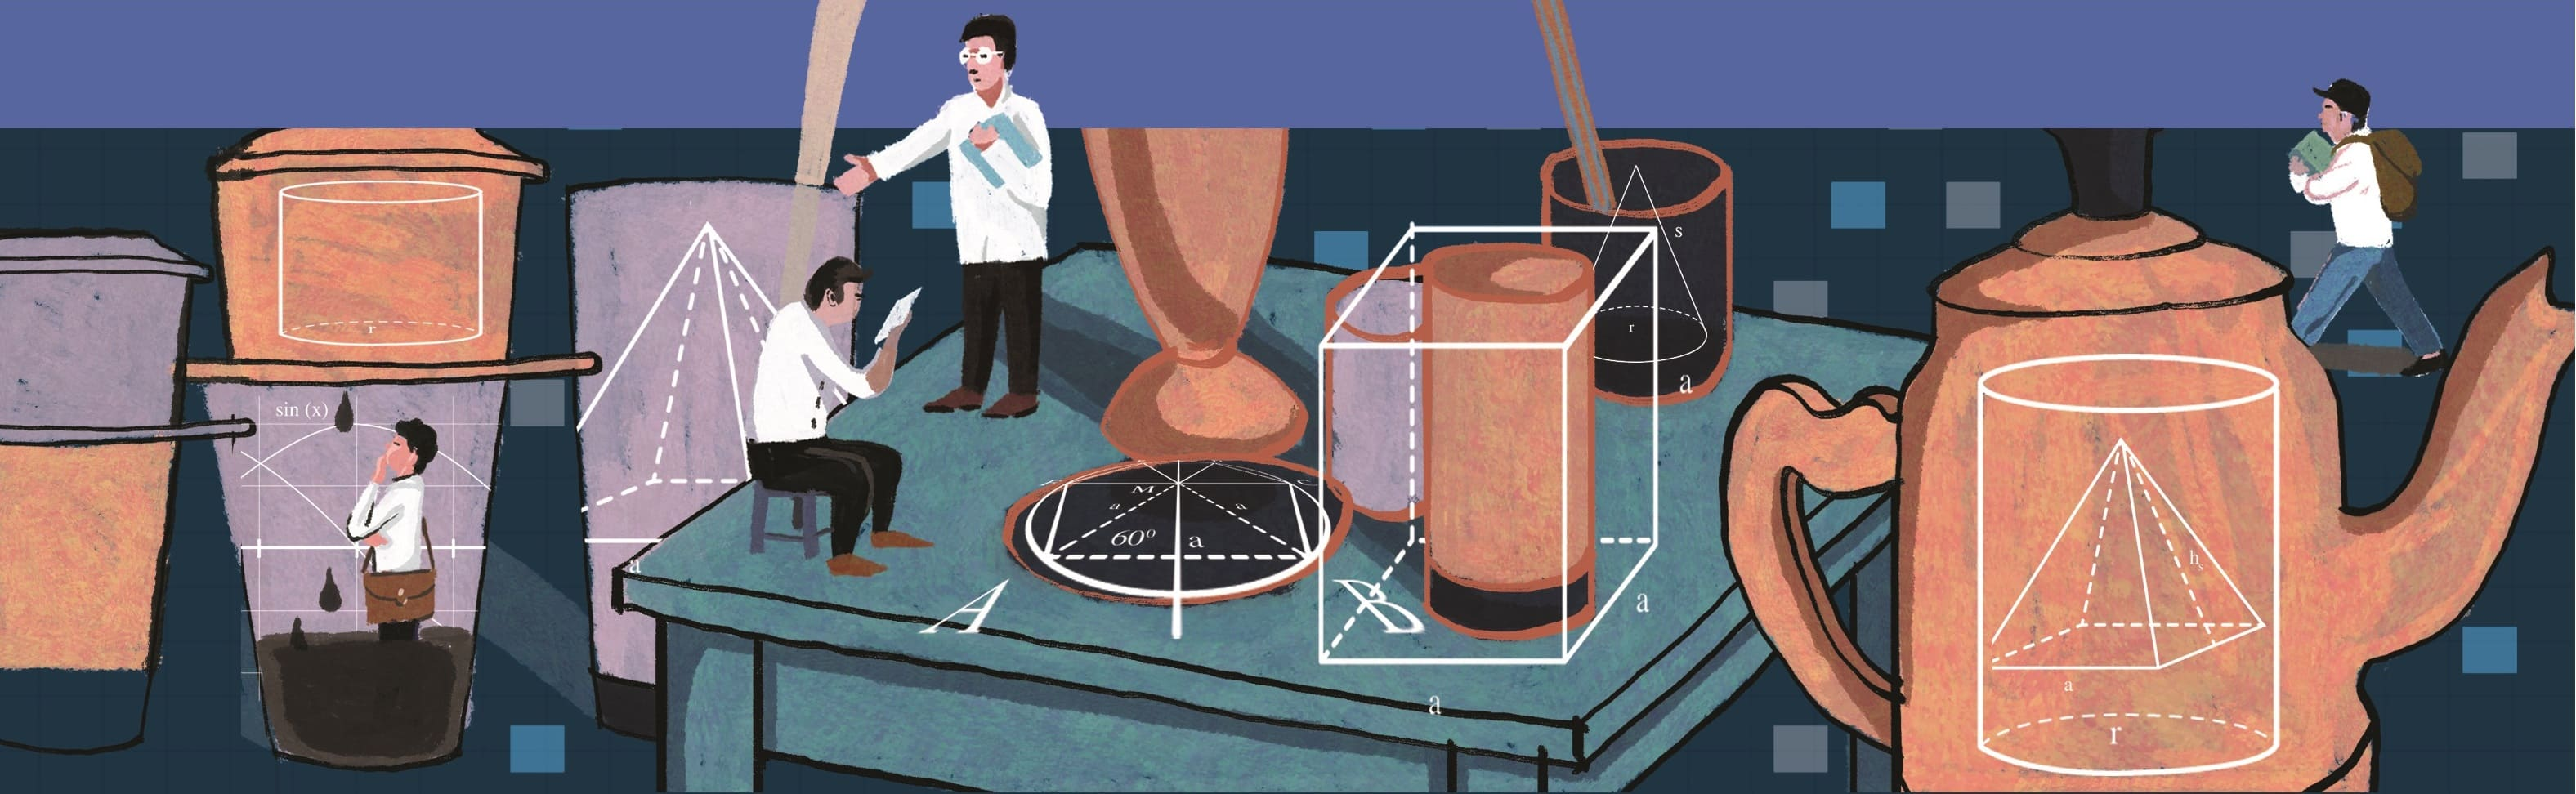
\includegraphics[width=19.3cm]{../bannerquantoan}}}
\AddToShipoutPicture*{\put(51,528){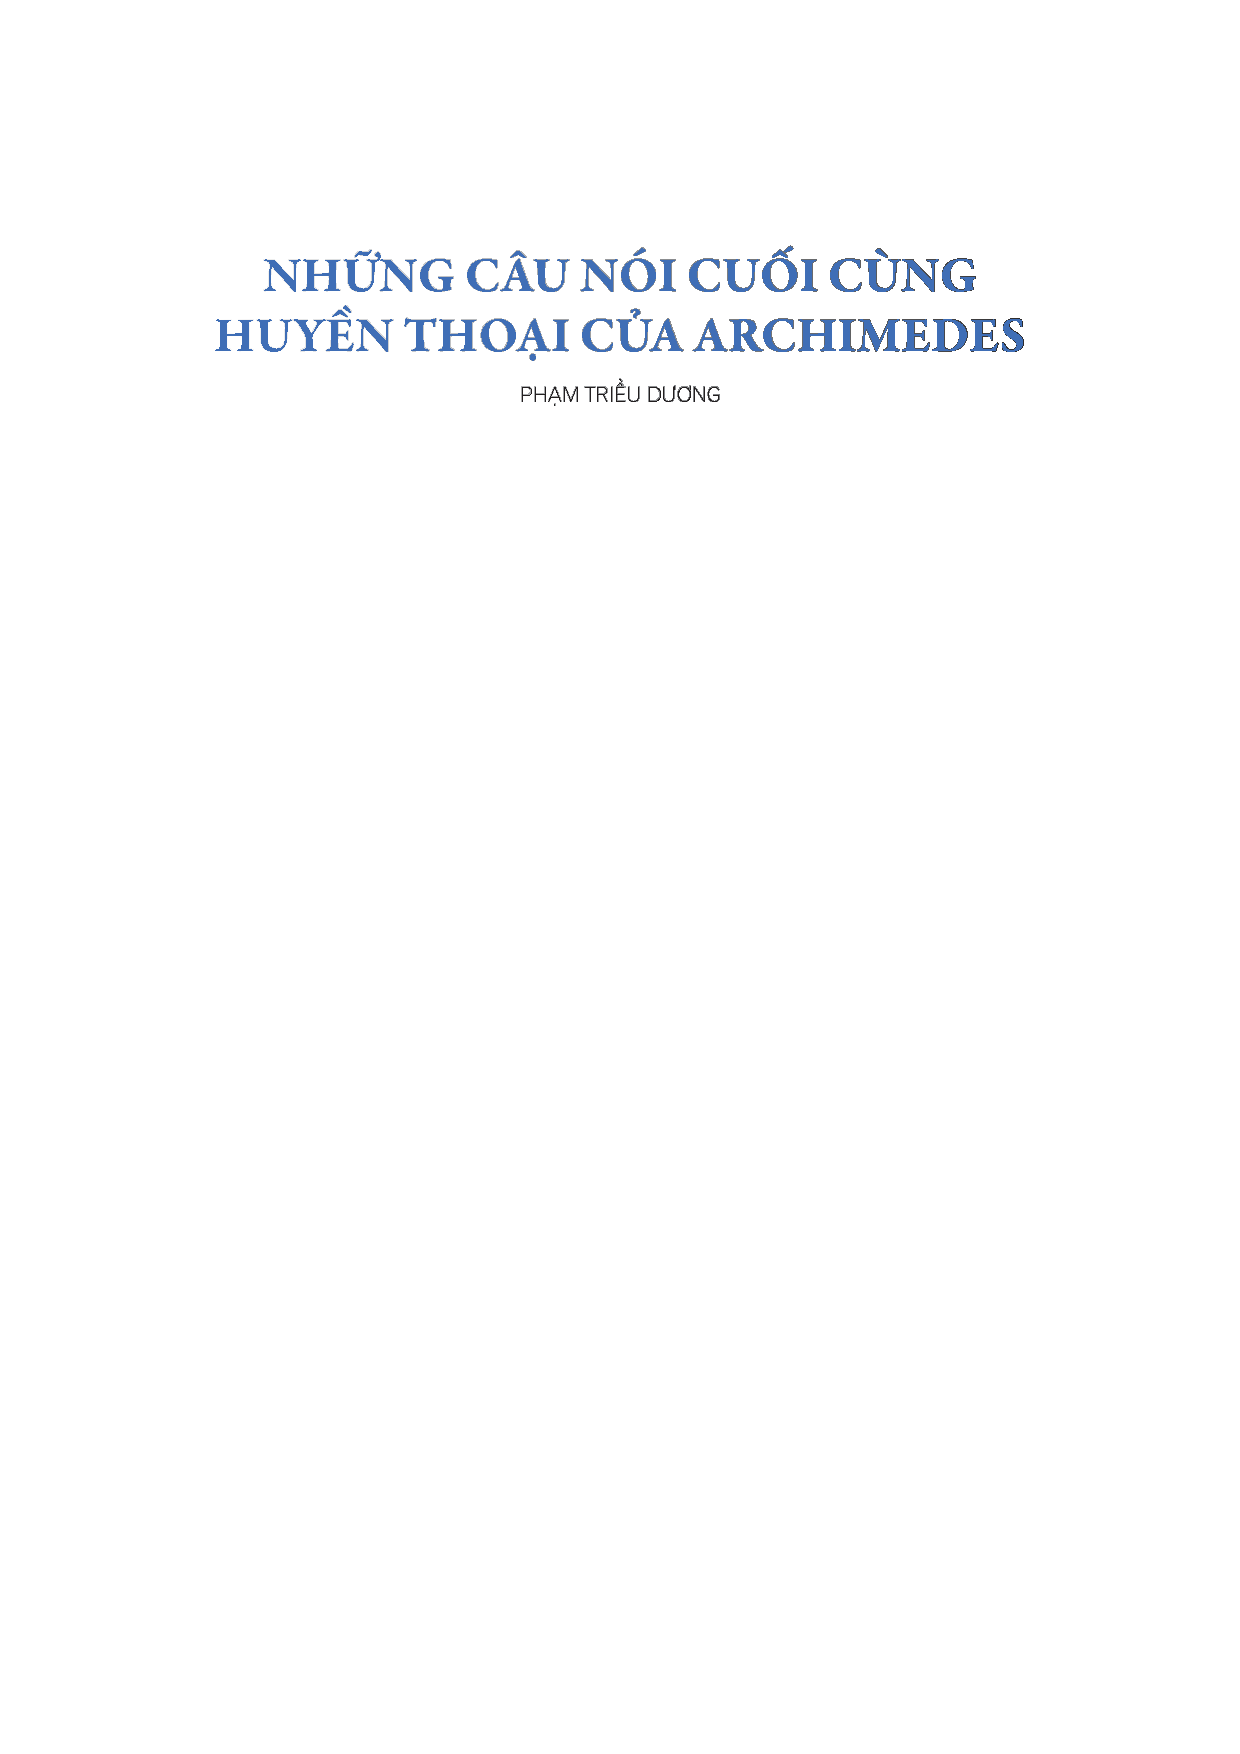
\includegraphics[scale=0.9]{../tieude1.pdf}}}
\centering
\endgroup

\vspace*{180pt}

\begin{multicols}{2}	
	Vladimir Igorevich Arnold ($1937-2010$) là một nhà toán học sinh ra ở Ukraine, người đã giành được giải thưởng Wolf cho công trình nghiên cứu về hệ động lực học, phương trình vi phân và lý thuyết kỳ dị. Niềm đam mê toán học của Arnold được bắt đầu khi ông mới $5$ tuổi. Ông giải thích trong [$2$] rằng đây là một hệ quả của truyền thống toán học Nga.
	\begin{figure}[H]
		\vspace*{-5pt}
		\centering
		\captionsetup{labelformat= empty, justification=centering}
		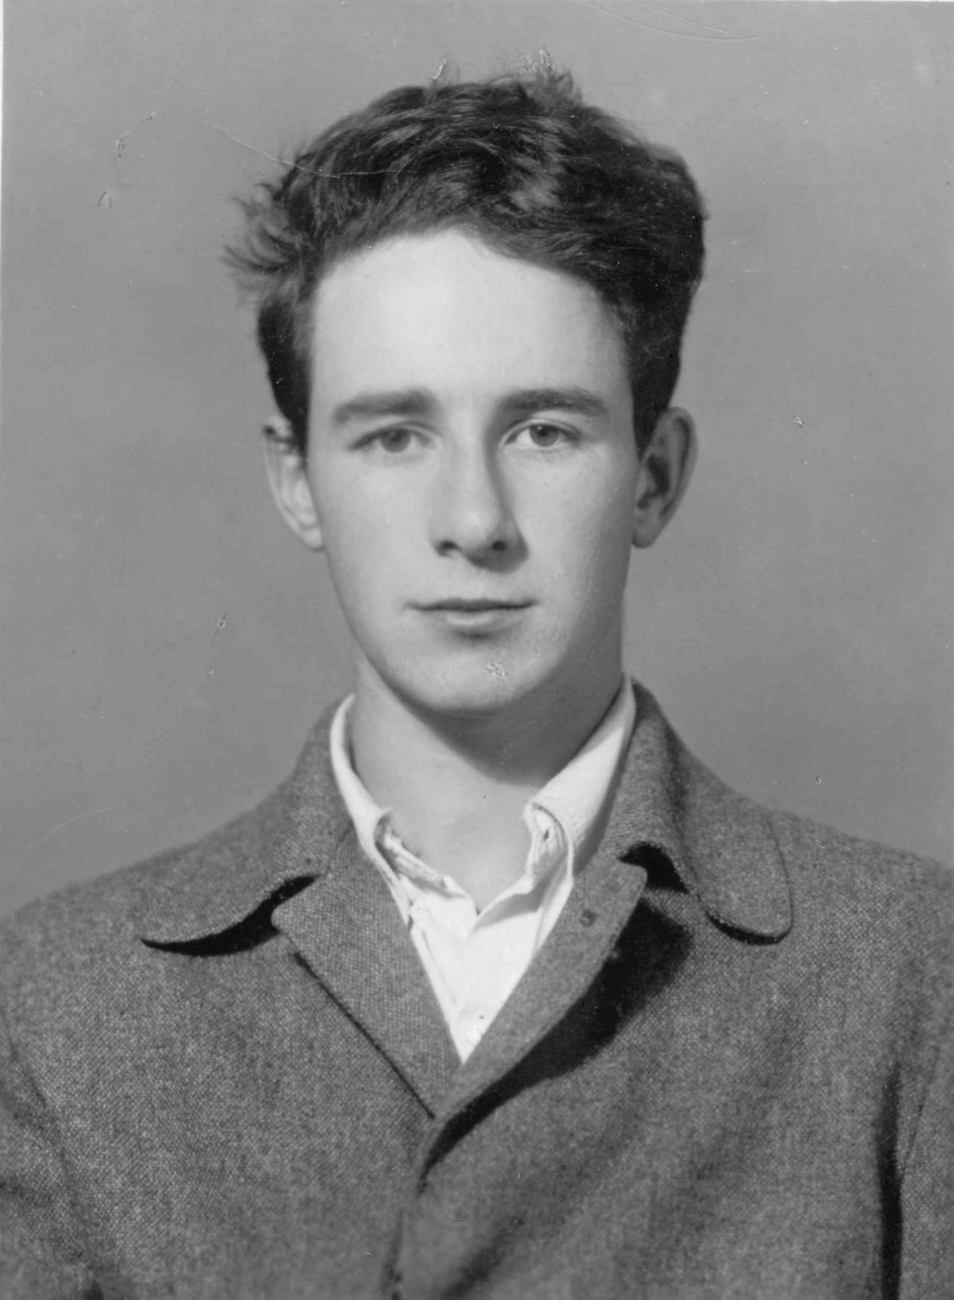
\includegraphics[width= 0.75\linewidth]{1}
		\caption{\small\textit{\color{quantoan}Vladimir Arnold vào năm $1957$.}}
		\vspace*{-10pt}
	\end{figure}
	\textit{Những  đứa trẻ khi còn rất nhỏ đã bắt đầu nghĩ về các bài toán (các bài toán cổ liên quan tới công việc buôn bán, trao đổi hàng hoá) ngay cả trước khi chúng có bất kỳ kiến thức nào về các con số. Trẻ em từ năm đến sáu tuổi rất thích các bài toán này và có thể giải được chúng, nhưng chính những bài toán đó lại có vẻ quá khó đối với những sinh viên tốt nghiệp đại học, những người đã bị làm hư bởi sự đào tạo toán học chính quy. ... Nhiều gia đình Nga có truyền thống đưa ra hàng trăm bài toán cho con cái của họ, và gia đình tôi cũng không ngoại lệ.}
	\vskip 0.1cm
	Khi mười hai tuổi, Arnold được thầy cô giáo  giao những bài toán khó. Ông trích dẫn một bài toán  như vậy trong [$2$]:
	\vskip 0.1cm
	\textit{Hai bà già bắt đầu đi từ lúc mặt trời mọc và mỗi người đi với vận tốc không đổi. Một người đi từ $A$ đến $B$ và người kia từ $B$ đến $A$. Họ gặp nhau vào giữa trưa và đi tiếp tục không nghỉ, lần lượt đến $B$ lúc $4$ giờ chiều,  và tới $A$ lúc $9$ giờ tối. Hỏi mặt trời mọc lúc mấy giờ vào ngày hôm đó?}
	\vskip 0.1cm
	Arnold thuật lại: 
	\vskip 0.1cm
	\textit{Tôi đã dành cả ngày để suy nghĩ về bài toán cũ kỹ đó, và lời giải ...  bỗng đến như một sự khám phá. Cảm giác khám phá mà tôi có lúc đó giống hệt như trong tất cả các bài toán nghiêm túc hơn nhiều về sau này ...}
	\vskip 0.1cm
	Là một nhà toán học nổi tiếng cả trong lĩnh vực nghiên cứu và giảng dạy, tuy nhiên Arnold luôn nhớ lại những năm tháng học đại học của mình với sự tôn trọng và đánh giá cao dành cho từng giáo sư được theo học và các bạn bè đồng môn. Ông kể lại trong [$2$]
	\vskip 0.1cm
	\textit{Sự quy tụ các ngôi sao toán học vĩ đại  trong cùng một khoa khi tôi theo học tại Khoa Toán -- Cơ là thực sự đặc biệt, và tôi chưa từng thấy điều gì giống như vậy ở bất kỳ nơi nào khác. Kolmogorov, Gelfand, Petrovsky, Pontryagin, P. Novikov, Markov, Gelfond, Lusternik, Khinchin và P. S. Aleksandrov lúc đó giảng dạy các sinh viên như Manin, Sinai, Sergei Novikov, V. M. Alexeev, Anosov, A. A. Kirillov và tôi. Tất cả những nhà toán học này đều rất khác nhau! Hầu như không thể hiểu được các bài giảng của Kolmogorov, nhưng chúng chứa đầy những ý tưởng và thực sự bổ ích! ... Pontryagin khi đó đã trở nên rất yếu lúc tôi là sinh viên của Khoa Toán Cơ, nhưng có lẽ ông ấy là giảng viên giỏi nhất của Khoa.}
	\begin{figure}[H]
		\vspace*{-5pt}
		\centering
		\captionsetup{labelformat= empty, justification=centering}
		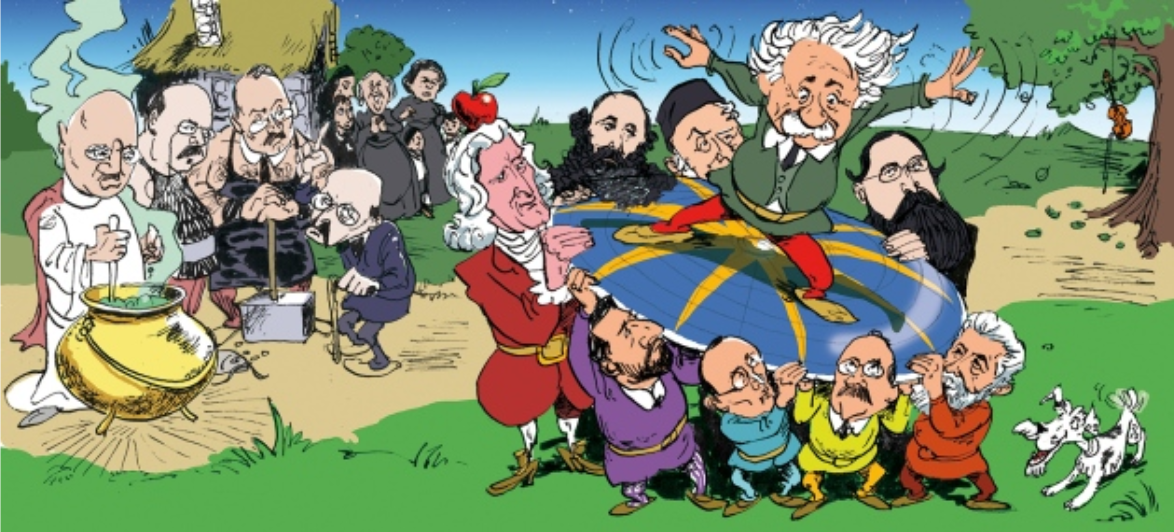
\includegraphics[width= 1\linewidth]{2}
		\caption{\small\textit{\color{quantoan}Thầy giáo Arnold cùng các học sinh Trường nội trú Toán Mátx--cơ--va vào những năm $1960$.}}
		\vspace*{-10pt}
	\end{figure}
	Năm $1965$, Arnold trở thành Giáo sư tại Khoa Toán -- Cơ tại Đại học Quốc gia Mát--xcơ--va, vị trí mà ông giữ cho đến năm $1986$ khi ông đảm nhận vị trí Nghiên cứu viên chính tại Viện Toán học Steklov ở Mát--xcơ--va. Ngoài các chức vụ ở Nga, năm $1993$, ông còn được bổ nhiệm làm Giáo sư tại Đại học Paris--Dauphine ở Pháp. Ông giữ chức vụ này cho đến năm $2005$.
	\vskip 0.1cm
	Khi nhận xét về cuốn sách Các bài toán của Arnold [$1$], Sergi Tabachnikov đã viết như sau trong [$4$] về các seminar của ông.
	\vskip 0.1cm
	\textit{Đời sống toán học ở Liên Xô từ cuối những năm $1950$, đặc biệt là ở Mát--xcơ--va, nổi tiếng với các seminar, như các seminar của Gelfand, Sinai, Kirillov, Manin, Novikov. Hầu hết các seminar này họp hàng tuần trong hai giờ, vào cuối buổi chiều. Đối với một số nhà toán học lỗi lạc, những seminar này là một cơ hội để thu hút và nuôi dưỡng những tài năng toán học mới chớm nở. Một trong những seminar nổi tiếng  là seminar của Arnold, tồn tại hơn $30$ năm. Mỗi học kỳ, buổi khai mạc của seminar luôn được dành cho các vấn đề mở. Arnold luôn trao đổi về hàng chục bài toán nghiên cứu với những bình luận chi tiết. Nhiều bài toán trong số này sau đó đã được giải quyết (hoặc giải quyết được một phần) bởi những người tham gia seminar. Theo Arnold, chu kỳ bán phân  rã của một bài toán là bảy năm. Nhiều người tham gia seminar cũng là nghiên cứu sinh của Arnold. Triết lý của ông luôn là: một sinh viên nên học được từ giáo viên của mình rằng một bài toán nào đó hiện đang là vấn đề mở; sự lựa chọn của một vấn đề nghiên cứu cụ thể sau đó là tùy thuộc vào sinh viên.}
	\begin{figure}[H]
		\vspace*{-5pt}
		\centering
		\captionsetup{labelformat= empty, justification=centering}
		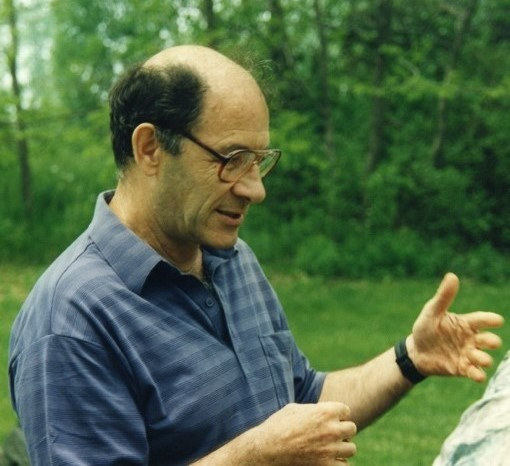
\includegraphics[width= 1\linewidth]{4}
		\caption{\small\textit{\color{quantoan}Vladimir Arnold vào năm $1997$.}}
		\vspace*{-10pt}
	\end{figure}
	Một cái nhìn tổng quan tuyệt vời về những đóng góp của Arnold đã được đưa ra trong phần trích dẫn về Giải thưởng Wolf được trao cho ông vào năm $2001$.
	\vskip 0.1cm
	\textit{Vladimir I. Arnold đã có những đóng góp đáng kể cho một số lượng đáng kinh ngạc các ngành toán học khác nhau. Nhiều công trình nghiên cứu, sách vở, bài giảng cộng với sự uyên bác và tâm huyết của ông đã có ảnh hưởng sâu sắc đến cả một thế hệ các nhà toán học. Luận án Tiến sĩ của Arnold có chứa một lời giải cho bài toán thứ $13$ của Hilbert. Công trình của ông về động lực học Hamilton, bao gồm việc đồng sáng tạo ra lý thuyết KAM (Kolmogorov--Arnold--Moser) và khám phá ra ``sự khuếch tán của Arnold", đã khiến ông nổi tiếng thế giới ngay từ khi còn nhỏ. Những đóng góp của Arnold cho lý thuyết kỳ dị bổ sung cho lý thuyết thảm họa của Thom và đã làm biến đổi lĩnh vực này. Arnold cũng đã có vô số đóng góp cơ bản cho lý thuyết phương trình vi phân, hình học symplectic, hình học đại số thực, phép tính biến phân, thủy động học và từ--thủy động học.  Ông thường phát hiện ra mối liên hệ giữa các vấn đề trong các lĩnh vực khác nhau.}
	\begin{figure}[H]
		\vspace*{-5pt}
		\centering
		\captionsetup{labelformat= empty, justification=centering}
		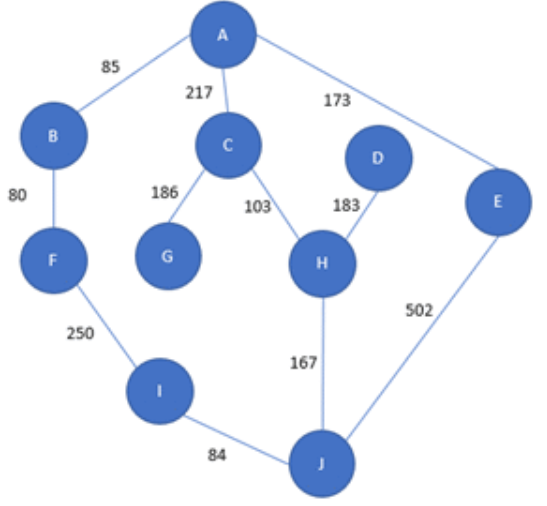
\includegraphics[width= 1\linewidth]{3}
		\caption{\small\textit{\color{quantoan}Giáo sư Arnold trong một buổi giảng bài.}}
		\vspace*{-10pt}
	\end{figure}
	Khi Arnold tròn $65$ tuổi vào năm $2002$, Tạp chí Toán học Mát--xcơ--va (Mát--xcơ--va Mathematical Journal) đã dành hai số báo để chào mừng sự kiện này với phần giới thiệu như sau: 
	\vskip 0.1cm
	\textit{...Bộ mặt của toán học hiện đại sẽ không thể nhận ra được nếu không có những công trình của ông trong các lĩnh vực như hệ động lực, cơ học cổ điển và cơ học thiên thể, lý thuyết  kỳ dị, tô pô, hình học đại số thực và phức, hình học symplectic và hình học tiếp xúc, thủy động học, phép tính biến phân, hình học vi phân, lý thuyết thế vị, vật lý toán học, lý thuyết chồng chất, v.v...
	\vskip 0.1cm
	Arnold là một giáo viên hiếm có, trường lớp của ông luôn nổi tiếng và đông đảo người theo, ông có năng khiếu đặc biệt trong việc tìm ra những vấn đề mới và  hấp dẫn để thu hút sự quan tâm và lôi cuốn các nhà nghiên cứu trẻ. Ông là một giảng viên phi thường ở tất cả các cấp giáo dục toán học và nghiên cứu. Những lý thuyết hiện đại khó hiểu trở nên khá rõ ràng và đơn giản trong phần trình bày của ông. Người ta khó có thể hình dung nền giáo dục toán học hiện đại nếu không có những cuốn sách giáo khoa xuất sắc của ông. Trường phái toán học Mát--xcơ--va phải mang ơn rất nhiều những seminar của ông.
	\vskip 0.1cm
	Xuất thân từ một gia đình nhiều thế hệ làm khoa học, ông tập hợp được cách tiếp cận khoa học của họ và mối quan tâm sâu sắc đến mọi mặt của cuộc sống, kiến thức của ông vô cùng rộng lớn và sự tò mò của Arnold đối với mọi thứ xung quanh thật tuyệt vời.}
	\vskip 0.1cm
	Arnold đã được trao Giải thưởng Nhà nước của Liên bang Nga ($2007$), và trong năm tiếp theo, ông đã nhận được Giải thưởng Shaw danh giá về khoa học toán học.
	\vskip 0.1cm
	Arnold đã có lần trả lời trong một bài phỏng vấn [$3$]: ``\textit{Người học không phải là chiếc túi phải lấp đầy, mà là ngọn đuốc cần được thắp sáng}".
	\vskip 0.1cm
	\textbf{\color{quantoan}Tài liệu tham khảo}
	\vskip 0.1cm
	[$1$] Vladimir I. Arnold (ed.). Arnold's Problems. \textit{Springer--Verlag, Berlin--Heidelberg--New York $\&$ PHASIS}, Mát--xcơ--va, $2005$, XV.
	\vskip 0.1cm
	[$2$]	S. H. Lui, An interview with Vladimir Arnold, \textit{Notices Amer. Math. Soc.} $44$ ($4$) ($1997$), $432-438$.
	\vskip 0.1cm
	[$3$]	S. Tabachnikov. Interview with V. I. Arnold. (\textit{in Russian}) \textit{Kvant} $1990$, No $7$, $2-7$, $15$.
	\vskip 0.1cm
	[$4$]	S. Tabachnikov. Arnold's Problems. \textit{The Mathematical Intelligencer.} $2007$
\end{multicols}
\newpage
\begingroup
\AddToShipoutPicture*{\put(132,678){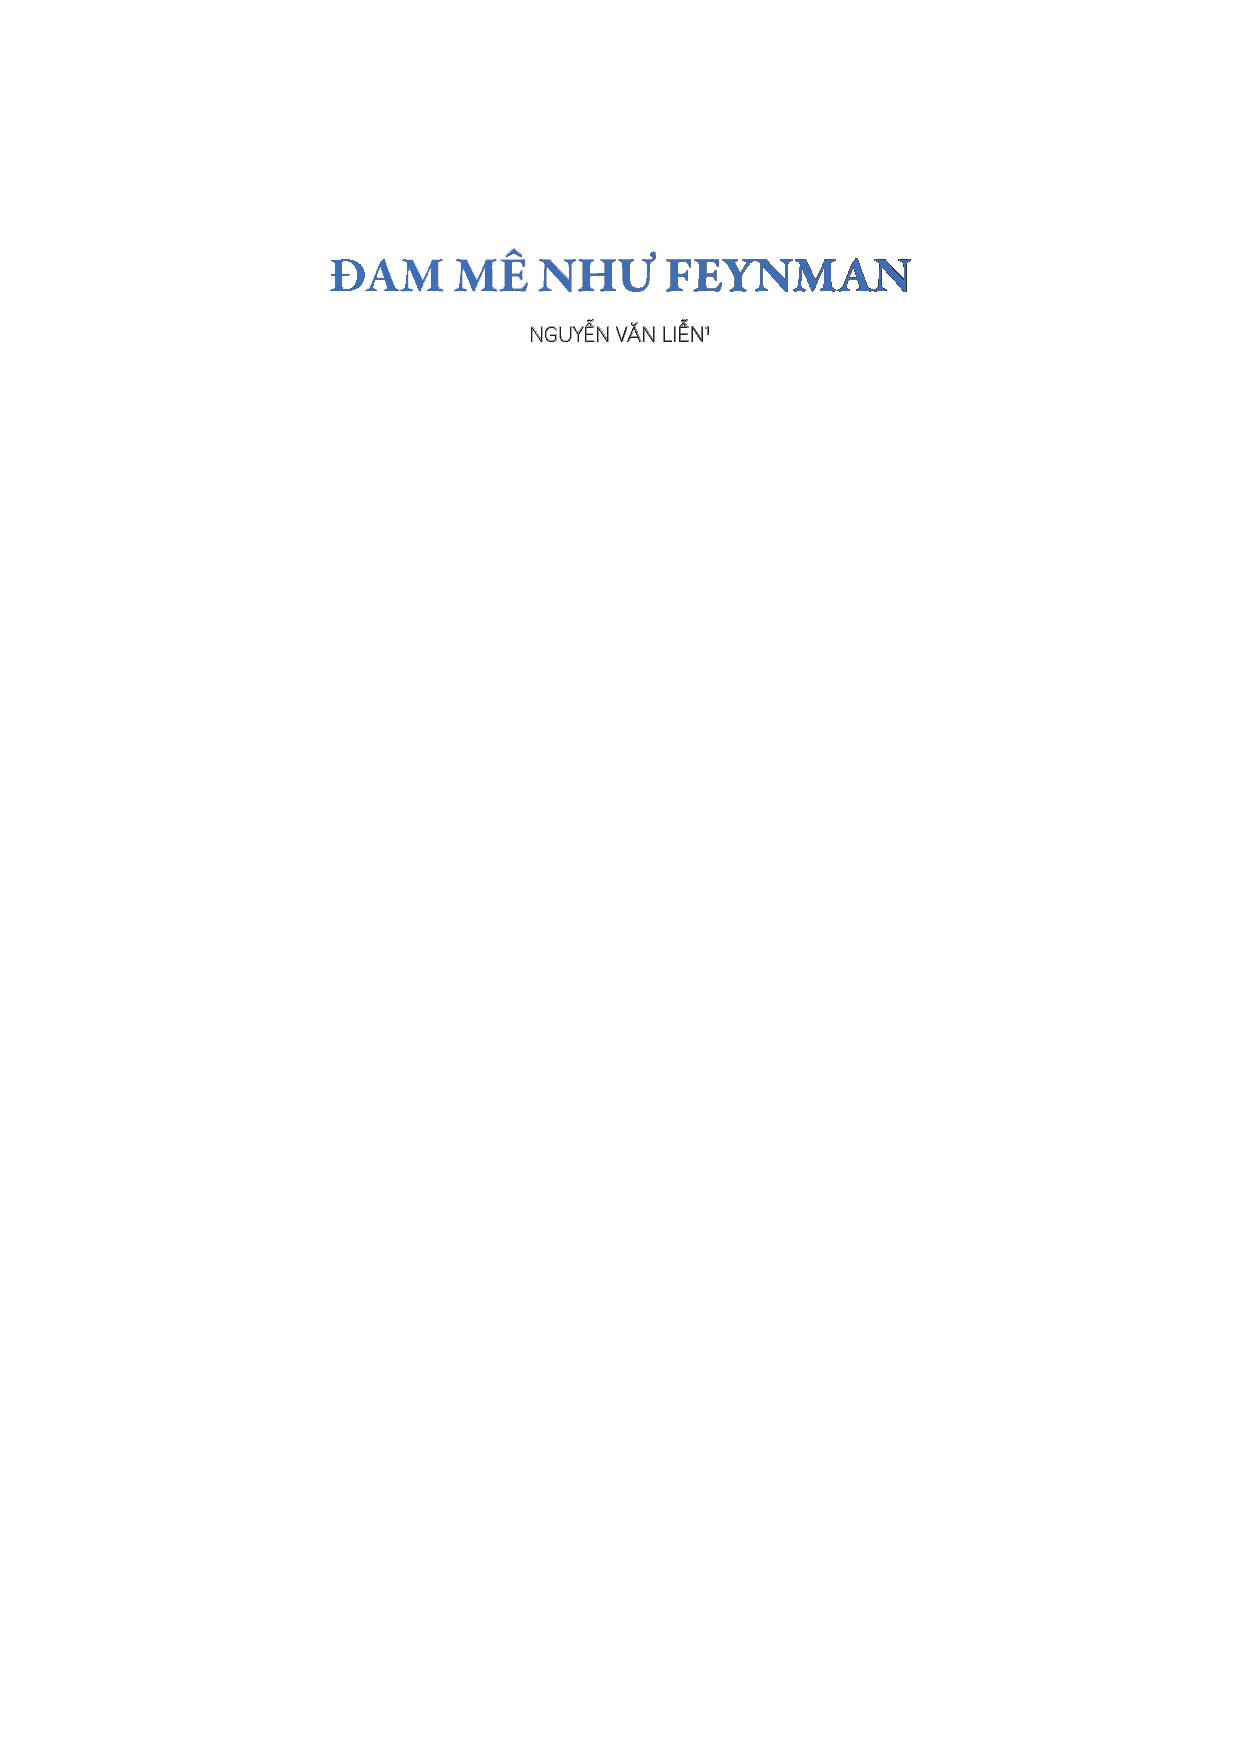
\includegraphics[scale=1]{../tieude2.pdf}}}
\centering
\endgroup
\blfootnote{$^1$\color{quantoan}Viện Vật lý.}
\vspace*{30pt}

\begin{multicols}{2}
	Richard Feynman ($1918-1988$, Mỹ) nổi tiếng là người trung thực không khoan nhượng và đam mê đến tận cùng. Về tính trung thực, người ta hay nhắc đến vụ ông trình diễn trực tiếp trên TV một ``thí nghiệm nhỏ", bỏ vòng cao su vào cốc nước đá, minh chứng rằng cao su mất tính đàn hồi ở nhiệt độ thấp, qua đó chỉ ra nguyên nhân dẫn đến thảm họa tàu vũ trụ con thoi ``Challenger", vạch trần chiến dịch tung hỏa mù của NASA về nguyên nhân của thảm họa này. Để công bố với người dân Mỹ sự thật ấy, Feynman đã phải vượt qua sức ép khủng khiếp từ các cơ quan công quyền Mỹ, trong đó có CIA và NASA. 
	\begin{figure}[H]
		\vspace*{-5pt}
		\centering
		\captionsetup{labelformat= empty, justification=centering}
		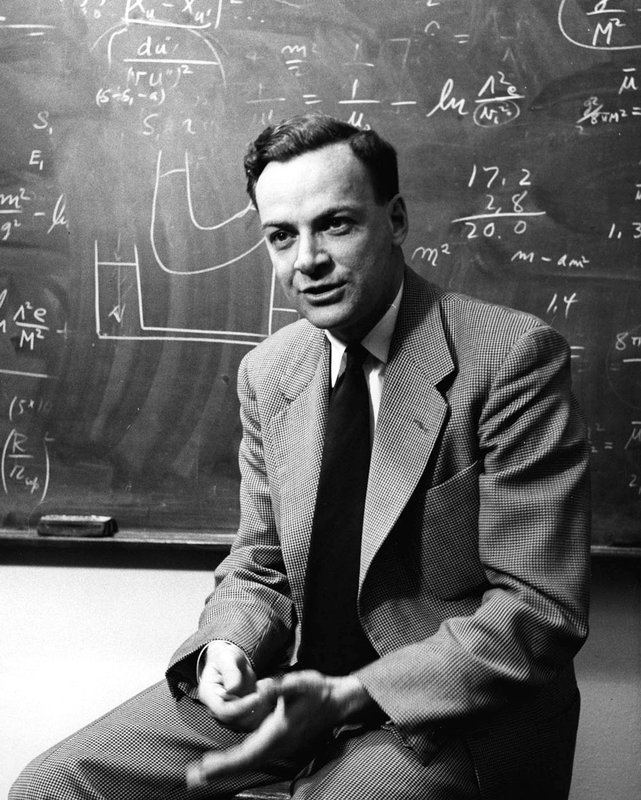
\includegraphics[width= 1\linewidth]{1a}
		\caption{\small\textit{\color{quantoan}Richard Feynman (ảnh từ bộ sưu tập của Viện Công nghệ California -- CalTech).}}
		\vspace*{-10pt}
	\end{figure}
	Feynman lắm đam mê. Đam mê vật lý, Feynman nhận giải Nobel Vật lý năm $1965$. Đam mê chơi trống, vở ba--lê do ông đệm trống nhận giải nhất trong cuộc thi ba--lê toàn nước Mỹ và giải nhì trong cuộc thi quốc tế tại Paris. Đam mê vẽ, ông đã có triển lãm tranh riêng. Không rõ ông biết những ngôn ngữ nào, chỉ biết thăm Brazil ông dạy bằng tiếng Bồ, thăm Nhật ông giao du bằng tiếng Nhật. Rồi có lần bạn bè định ``cho ông một vố", họ nhờ một cô Hoa kiều đón tiếp ông bằng tiếng Trung, Feynman đáp lại và cô ấy kêu trời, vì ông nói tiếng Quảng Đông, còn cô chỉ nói tiếng Bắc Kinh. Rất nhiều ``đam mê" kiểu như vậy được kể trong cuốn ``Feynman, chuyện thật như đùa" (NXB Trẻ) và hầu như tất cả đều có kết cục mỹ mãn, kiểu như giải Nobel. Có thể bạn nghĩ chắc ông này ``con nhà nòi", học ``trường quốc tế" từ nhỏ! Xin thưa, bố của Feynman là người bán rong bán quần áo, còn mẹ thì nội trợ. 
	\begin{figure}[H]
		\vspace*{-5pt}
		\centering
		\captionsetup{labelformat= empty, justification=centering}
		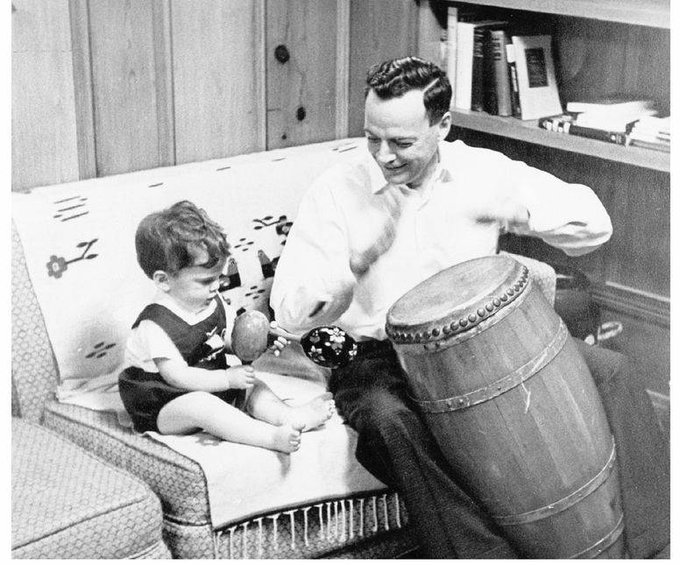
\includegraphics[width= 1\linewidth]{2a}
		\caption{\small\textit{\color{quantoan}Feynman chơi trống bên con trai (ảnh từ Internet).}}
		\vspace*{-10pt}
	\end{figure}
	Ông chơi trống bongo cực giỏi, nhưng chưa bao giờ học nhạc lý. Ông vốn vẽ rất kém, tự nhận chẳng thể vẽ nổi cái gì ngoại trừ cái kim tự tháp chỉ gồm mấy đường thẳng. Để học vẽ, Feynman ``đổi công" với một họa sỹ: ông dạy vật lý cho họa sỹ còn họa sỹ dạy vẽ cho ông. Hãy tưởng tượng một giáo sư nổi tiếng thế giới ngồi trong lớp vẽ cùng các cháu $8-9$ tuổi học cách gọt bút chì. Đam mê như thế chỉ có ở Feynman. Và, với ông đam mê chính là nguồn cội của thành công, chứ chẳng phải ``con nhà nòi" hay ``trường quốc tế" nào cả. Tiền bạc và chứng chỉ đầy người, mà không đam mê gì, thì làm sao có thành quả! 
	\begin{figure}[H]
		\vspace*{-5pt}
		\centering
		\captionsetup{labelformat= empty, justification=centering}
		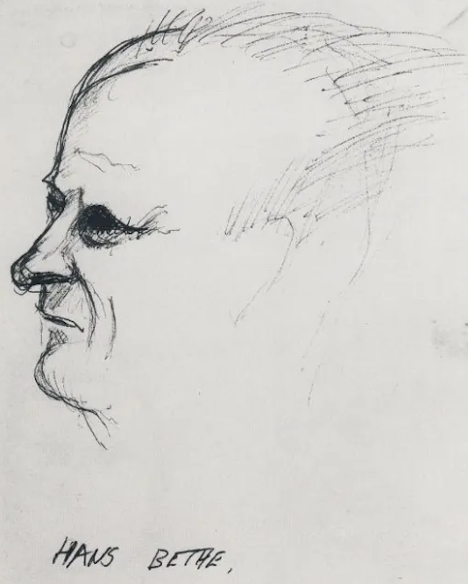
\includegraphics[width= 1\linewidth]{3a}
		\caption{\small\textit{\color{quantoan}Feyman vẽ Hans Bethe (giải Nobel Vật lý $1967$).}}
		\vspace*{-10pt}
	\end{figure}
	Duy có đam mê cuối cùng, Feynman đã không kịp nhìn thấy những gì mình muốn, trước khi về cõi vĩnh hằng. Đó là ``Cuộc phiêu lưu cuối cùng của Feynman"\footnote[2]{\color{quantoan}Xem thêm: Cuộc phiêu lưu cuối cùng của Feynman, in lần $2$, NXB Trẻ, $2023$.}. Cuộc phiêu lưu khởi đầu bằng một con tem có xuất xứ từ một nơi gọi là Tannu Tuva, mà Feynman có được từ khi còn nhỏ. Cái tên ``Tuva" xa lạ nằm yên trong đầu Feynman, cho đến một ngày hè $1977$ nó trở thành mục tiêu cho ``cuộc phiêu lưu" kéo dài hơn $10$ năm cuối của cuộc đời ông. Tôi cược là nhiều bạn chưa biết Tuva là địa danh nào và ở đâu. Để đỡ tra cứu, xin ``bật mí" ngay: đó là tên một quốc gia nhỏ nằm giáp phía Tây Bắc của Mông Cổ, vốn độc lập, nhưng đã sáp nhập vào Liên Xô cũ (và Nga ngày nay). Thủ đô của Tuva là Kyzyl. Tuva có gì đặc biệt mà khiến Feynman mê mệt đến vậy?
	\vskip 0.1cm
	Bạn có biết đâu là trọng tâm của châu Á (lục địa thôi chứ không tính các đảo)? Lấy tấm bìa cứng phẳng, vẽ lên đó bản đồ châu Á, cắt theo đường biên để được miếng bìa hình châu Á lục địa. Dùng một chiếc bút đầu nhọn chống phía dưới tấm bìa, di di đầu bút, để tìm vị trí mà tấm bìa nằm cân bằng trên chiếc bút thẳng đứng. Vị trí đó rơi vào Kyzyl, trọng tâm của châu Á. Tất nhiên, các nhà khoa học xác định điểm này bằng các phương pháp chính xác hơn, và ngày nay ở Kyzyl có tấm bia lớn khẳng định vị trí đặc biệt của thành phố này. Nhưng, chỉ chừng ấy thì không đủ để Feynman mất tới cả chục năm tìm cách tới thăm Tuva.
	\begin{figure}[H]
		\vspace*{-5pt}
		\centering
		\captionsetup{labelformat= empty, justification=centering}
		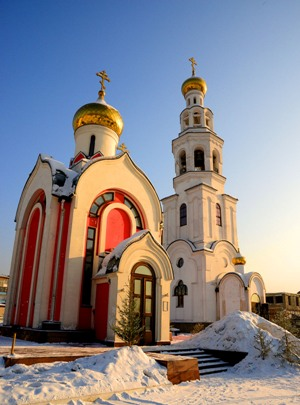
\includegraphics[width= 1\linewidth]{4a}
		\caption{\small\textit{\color{quantoan}Nhà thờ Phục sinh ở Kyzyl, Tuva (ảnh từ Internet).}}
		\vspace*{-10pt}
	\end{figure}
	Cái chính là ở quốc gia tí xíu bao bọc bởi những dãy núi cao ấy, thời gian gần như ngừng trôi: tất cả vẫn nguyên sơ như $500$ hay $1000$ năm trước. Thảo nguyên hoang dại. Những đàn tuần lộc hay bò Tây Tạng cũng dường như hoang dại. Cuộc sống du mục không thể tự nhiên hơn. Một nền văn hóa xa xưa và kỳ thú với kiểu hát hai giọng chỉ có ở Tuva, với thứ văn tự không thể tìm thấy trong bất cứ tự điển nào, với các tập tục rất lạ điều hành bởi các tù trưởng uy nghi và bí ẩn v.v. Tiếc là ít người biết Tuva, chứ không, người ta đã gọi quốc gia này là ``Thảo nguyên Xanh" cuối cùng của hành tinh Trái Đất (như Congo là Hành tinh Xanh cuối cùng). Đam mê Tuva, Feynman tìm đọc mọi tài liệu về Tuva, tìm hiểu văn tự Tuva, học cách hát của dân du mục Tuva, ăn mặc và trang trí như tù trưởng Tuva \ldots Và, nhất là, ông tìm mọi cách để có thể đến thăm Tuva.
	\vskip 0.1cm
	Đó là thời Chiến tranh Lạnh, lại nghe nói, gần Tuva có một cơ sở nghiên cứu bom nguyên tử, nên nơi đây là ``vùng cấm" với khách du lịch, nhất là khách nước ngoài. Thực ra, Viện Hàn lâm Khoa học Liên Xô sẵn sàng mời Feynman sang Moscow  đọc bài giảng rồi đi ``tham quan Kyzyl" theo kiểu mặc com--lê ở khách sạn có người bảo vệ v.v. Nhưng Feynman không thích như vậy, mà muốn tự mình mang ba--lô đến thảo nguyên, ngủ lều, uống sữa tuần lộc và hát hai giọng cùng dân bản xứ. Ấy thế cho nên ông mất cả chục năm tìm kiếm một giấy mời như mình muốn. Và, đầu tháng Ba $1988$, một giấy mời như thế đã gửi đến địa chỉ của Feynman, chỉ tiếc là hai tuần trước đó, vào ngày $15$ tháng Hai, ông đã ra đi mãi mãi, nên chỉ có thể trải nghiệm ``Cuộc phiêu lưu cuối cùng" của mình trong tâm trí và trái tim của những người ở lại. Không rõ, ở Thế giới bên kia Feynman đang đam mê gì?
\end{multicols}